% !TEX root = ./../../_Thesis.tex

% section's Name and Label
\section{The Human Eye}
\label{sec:TheHumanEye}

The eye is a sophisticated imaging system capable of dynamically adjusting its refractive power to focus at a wide range of depths. Optical aberrations in this imaging system are the main causes of loss of visual acuity. {\it Visual acuity} (\ie, the eye's ability to see fine details) can be determined with an auxiliary chart, in which the individual must resolve its details (\eg, bars and gaps) to recognize targets, such as Snellen or Sloan letters (Figure \ref{fig:visual_acuity}). The ability to distinguish between two details determines the {\it Minimum Angle of Resolution} (MAR). The standard visual acuity for humans is 1 arc minute (one-sixtieth of one degree) \cite{Schwartz2010}. In ophthalmology, visual acuity is commonly recorded in the form of the {\it Snellen fraction}: $VA = D'/D$, where $D'$ is the standard viewing distance (usually 20 feet) and $D$ is the distance at which each letter in the chart line subtends 5 arc minutes. The larger the $D$ value, the worse the vision. The term 20/20 vision is the standard for emmetropes (\ie, at a 20 feet distance, a person with normal vision should be able to read the small 20/20 line on an eye chart).

\begin{figure}[h]

	\centering
	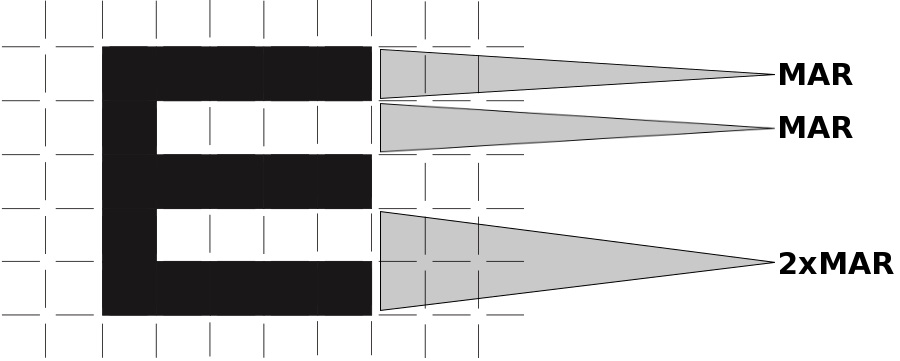
\includegraphics[width=1.0\linewidth]{__Images/02/e_optotype.png}
	\caption[Construction of the optotype E]{Construction of the optotype E. The detail (a bar or a gap) is one-fifth of the overall size of the optotype. MAR stands for Minimum Angle of Resolution, which corresponds to 1 arc minute. Modified from \citet{Schwartz2010}.}
	\label{fig:visual_acuity}
\end{figure}